\chapter{Лекция 1. Введение}

\section{О преподавателе}

Дмитрий Юрьевич Булычев

email: dboulytchev@math.spbu.ru

phone: +7-911-921-08-19

\section{Введение в предмет}

\paragraph{Из истории.} Первый язык программирования высокого уровня Fortran появился в 1957 году, до этого пользовались языками ассемблера и машинными кодами.
Вся история развития языков программирования связана с повышением уровня абстракции языков. От Fortran-а следующим повышением уровня стали процедурные языки
(Алгол-60), которые предоставляли средства структуризации программ. Первый объектно-ориентированный язык программирования Симула-67, далее уже появился знаменитый
Smalltalk. Вначале процедурные и объектно-ориентированные языки развивались параллельно, но процедурные языки являлись мейнстримом, по мере развития акцент смещался
от процедурных к объектно-ориентированным.

\paragraph{Составляющие языка программирования:}

\begin{itemize}
\item Синтаксис языка (правила записи правильных языковых конструкций). Синтаксис бывает двух форм: абстрактный и конкретный. Пример ниже, представление программы в
некотором конкретном синтаксисе, но для оперирования с программой требуется некоторая абстракция или абстрактный синтаксис.

\begin{lstlisting}
int f(int n) {
	if (n == 0) return 1;
	return n*f(n-1);
}
\end{lstlisting}
\label{code::code1}

Эта же программа в некотором абстрактном синтаксисе может выглядить так:

\begin{figure}
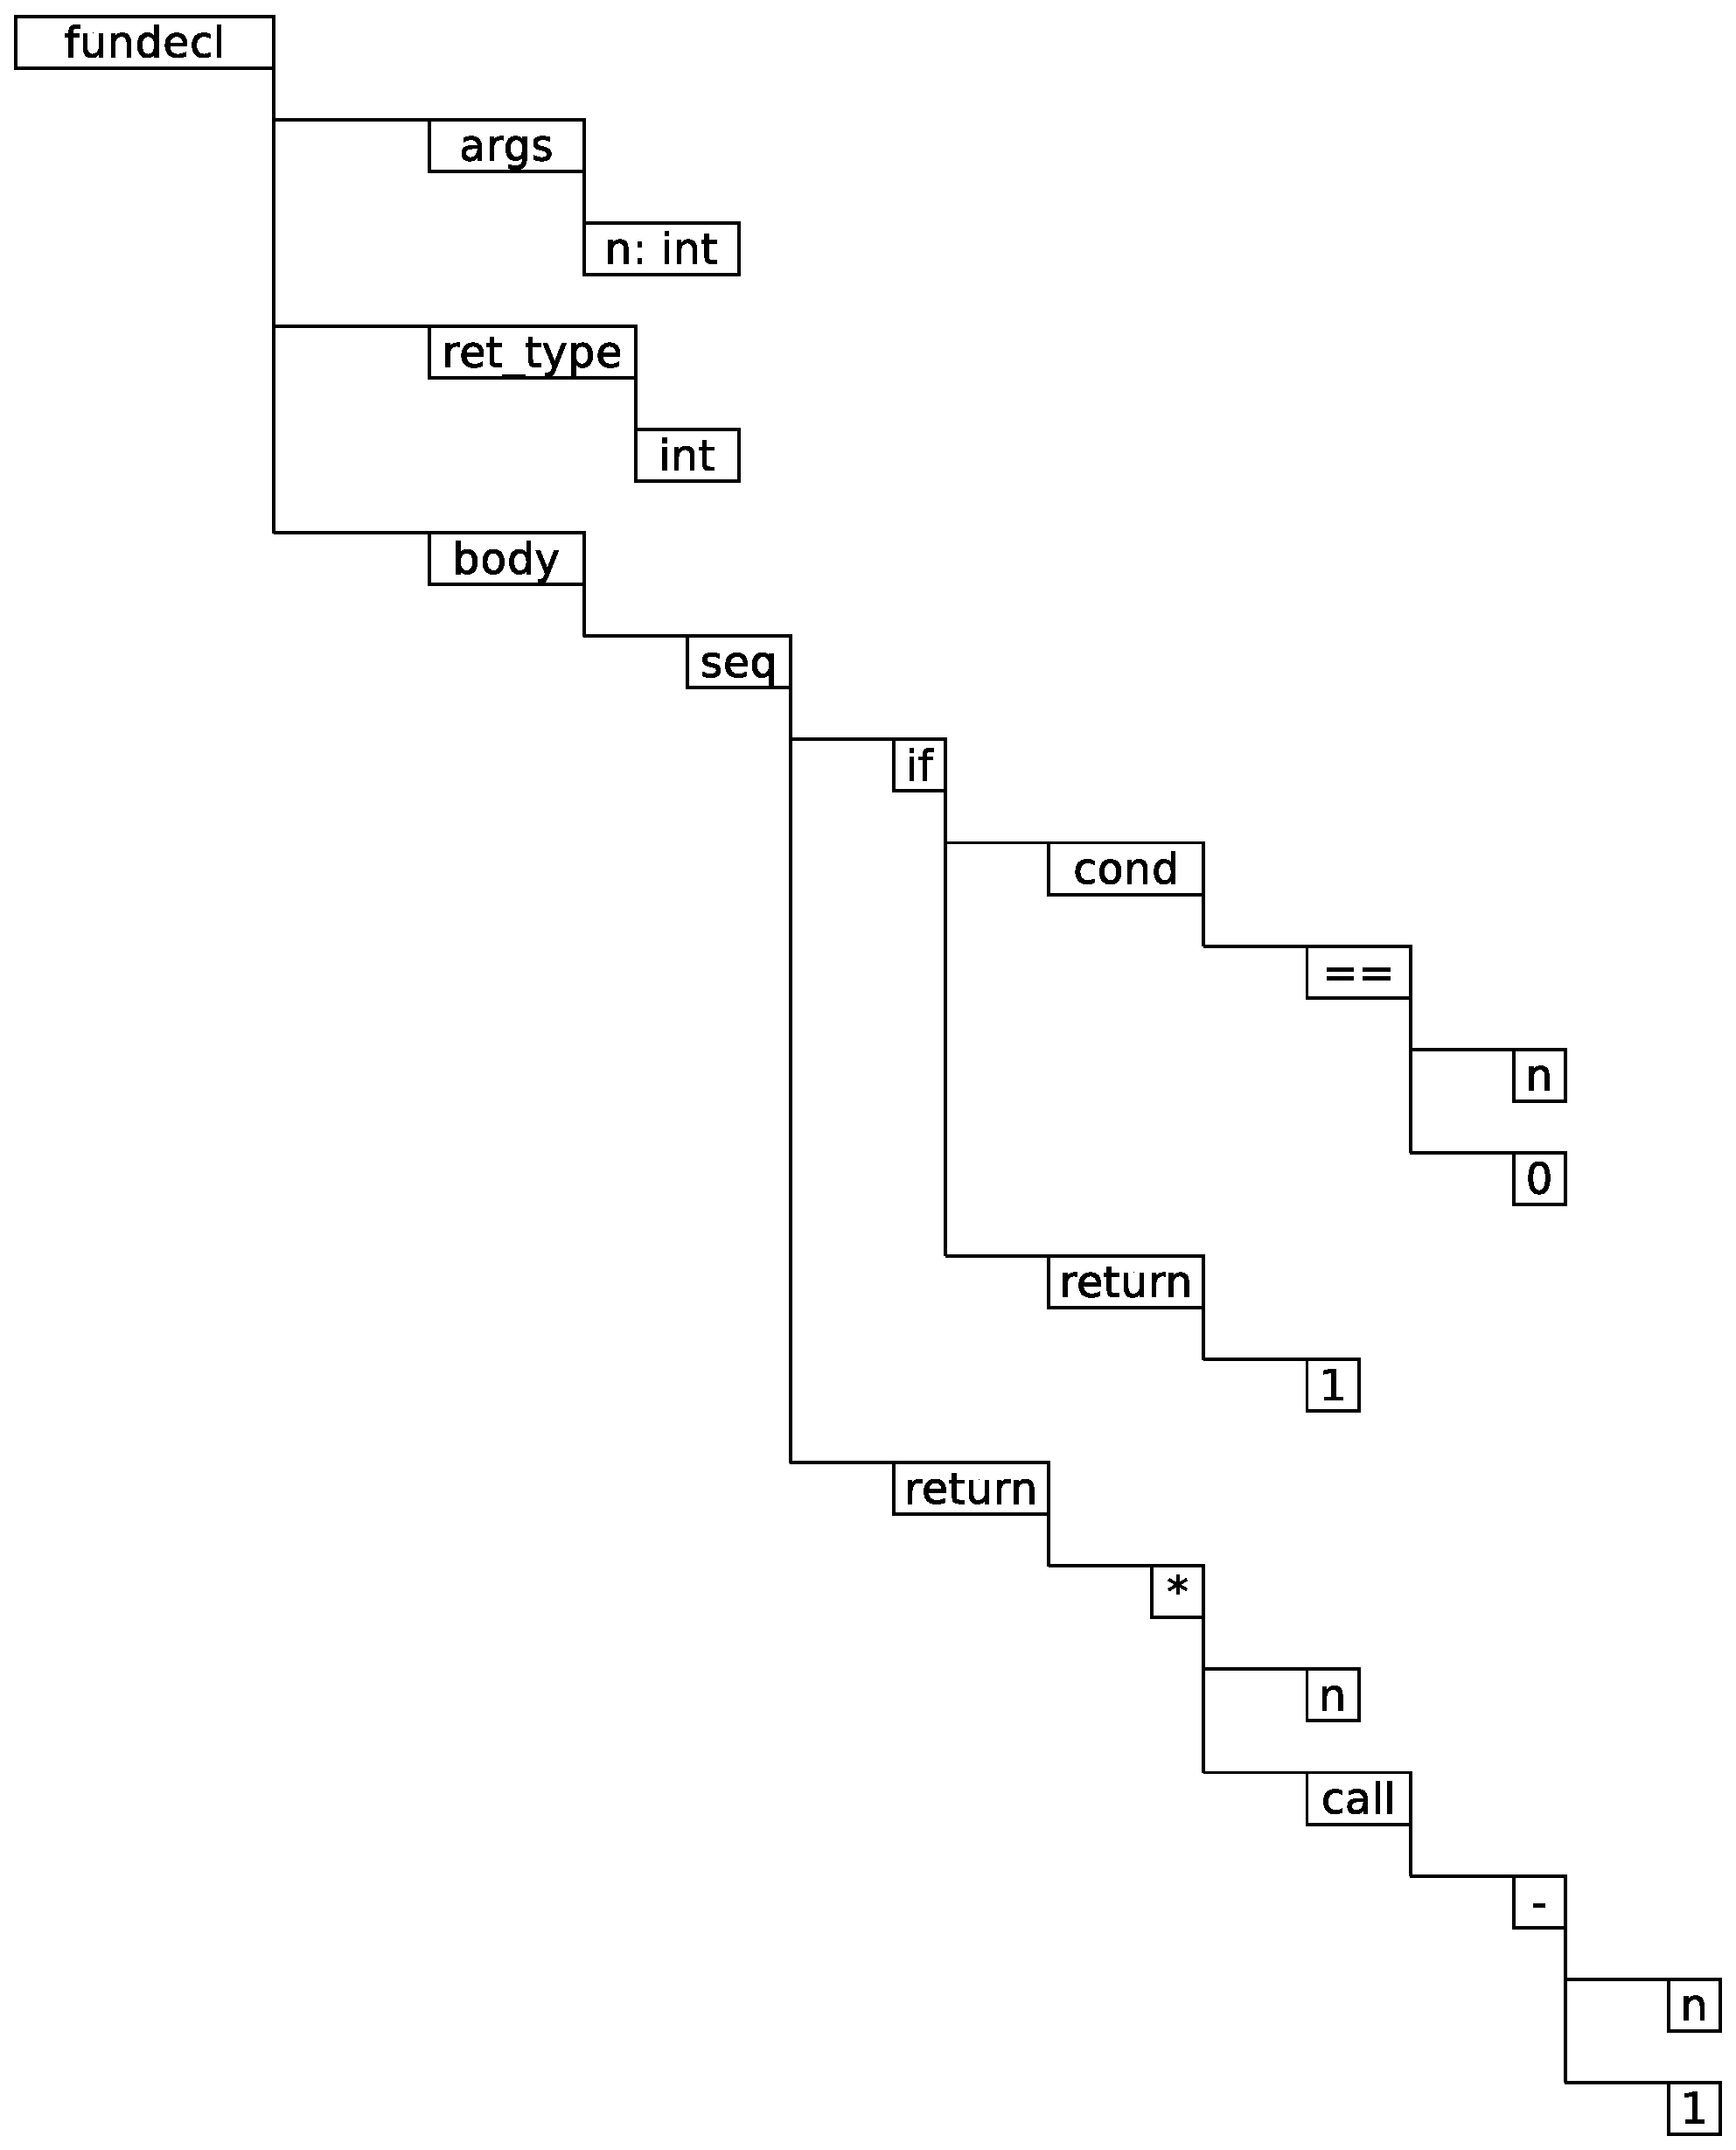
\includegraphics[width=\linewidth]{img1}
\caption{Абстрактное синтаксическое дерево программы \ref{code::code1}}
\label{img::img1}
\end{figure}

т. е. представление в абстрактном синтаксисе это некоторая иерархическая структура (дерево). Абстрактный синтаксис является некоторой моделью языка
программирования.

\item Семантика - некоторое отображение, сопоставляющее программе некоторую функцию на совокупности данных (если очень неформально). Т. е. каждая программа
берет какие-то данные и получает результат, таким образом реализует функцию: $$ \mathbb{S}_L : \mathbb{P}_L \rightarrow \left(D \hookrightarrow D\right) $$

где $\mathbb{S}_L$ - семантика (динамическая) языка $L$, а $\mathbb{P}_L$ - множество всех программ данного языка $L$, а $\left(D \hookrightarrow D\right)$
частично-определенное отображение из множества данных в множество данных. Семантика может и не быть определена для некоторой программы.

Семантика бывает статической и динамической. Статическая семантика является чисто прикладной вещью, позволяющей отбросить заранее плохие программы (например,
программа с неопределенной семантикой), или чтобы получать более эффективную программу. Статическая семантика - некоторый предикат заданный на программе.

\item Прагматика - типичные правила использования. Паттерны, хороший стиль программирования и прочее, все это есть прагматика языка. Данный раздел не поддается
формализации.
\end{itemize}

\paragraph{Примеры объявлений на СИ:}

\begin{itemize}
\item int (*f(int arg))(int, int) - прототип функции f, которая принимает int, а возвращает указатель на функцию принимающую два int и возвращающее int

\item typedef int (*fp)(int, int) - описание синонима fp для типа указателя на функцию, принимающую два int и возвращающую int
\end{itemize}

написать такие вещи трудно не пользуясь некоторыми формальными правилами, но если такие знать такие правила, можно писать действительно сложные конструкции.
В данном случае правило можно сформулировать так: объявляй типы так как потом будешь их использовать. Понятно, что такие конструкции используются достаточно
редко, это пример того, что прагматика языка гораздо меньше возможностей самого языка.

Другой пример таких тонкостей, но уже более полезный:
\begin{lstlisting}
do {
	...
} while(0)
\end{lstlisting}
где такое может понадобится? Ответ в макросах, например:
\begin{lstlisting}
#define makeIt(x) S1(x); S2(x)

if (?) makeIt(x);
\end{lstlisting}
в таком виде после раскрытия макроса получаем:
\begin{lstlisting}
if (?) S1; S2;
\end{lstlisting}
очевидно, это неправильно, скажем а почему просто не встатить ${}$? вот другой пример:
\begin{lstlisting}
if (?) makeIt(x); else ...
\end{lstlisting}
который преобразуется в этом случае:
\begin{lstlisting}
if (?) {S1(x);S(2)}; else ...
\end{lstlisting}
опять получаем ошибку, в самом идеальном случае надо пользоваться следующим макросом:
\begin{lstlisting}
#define makeIt(x) do {int y = x; S1(y); S2(y)} while(0)

if (?) makeIt(x); else ...
\end{lstlisting}

\section{Операционная семантика языков}

Теперь познакомимся с некоторыми интересными вещами, на не очень формальном уровне. Операционная семантика - это семантика, которая задается или определяется
эталонным интерпритатором (написать некоторый интерпритатор значит задать семантику (динамическую)).

Пусть имеется язык $L$, как задать его семантику? Ответ, написать программу-интерпритатор, которая пройдет эту программу по шагам и выполнит все действия.
Например, возьмем программу \ref{code::code1}, точнее ее абстрактное синтаксическое дерево. Программа проходящая по этому дереву \ref{img::img1},
исполняя его узлы и будет тем самым интерпритатором, во время написания интерпритатора мы опишем и семантику языка. Эталонный интерпритатор - некоторый
интерпритатор работа которого считается правильной. Имеем: $$ I^L : L \rightarrow \left(D \hookrightarrow D\right) $$ или в других обозначениях:
$$ I^L \left(p_L \in L, x\right) = p_L\left(x\right) $$
где $p_L$ - программа на языке $L$, а $p_L(x)$ - применение семантики программы $p_L$ к данным $x$.

Тут есть некоторая тонкость, $I$ - тоже программа, она может быть написана как на языке $L$, так и на другом языке $T$, в полных обозначениях имеем $I^L_T$, где
$T$ - язык описания интерпритатора.

Интерпритатор должен быть всюду определен, т. е. для любого абстрактного синтаксического дерева допустимого языком $L$ интерпритатор $I^L$ должен быть определен.

Создание интерпритатора - конструктивный способ задания семантики, но не единственный. Пример реального использования этих вещей - JavaVM, все сертифицированные
Java машины обладают одинаковой семантикой.

\paragraph{Отступление.} Пусть имеется функция двух аргументов $f\left(x,y\right)$. Будем обозначать $f_a\left(y\right) = f\left(a,y\right)$ - эта фиксация
называется специализацией. Каждую такую вычислимую функцию можно занумеровать, причем по номеру $f\left(x,y\right)$ и параметру $a$ можно посчитать номер функции
$f_a\left(y\right)$, таким образом построение специализации можно сделать автоматически, то есть существует функция, которая сделает по функции $f\left(x,y\right)$
и некоторому параметру $a$ ее специализацию $f_a\left(x\right)$, такая функция называется специализатором: $$ Mix^L : L \rightarrow D \rightarrow L $$ или в других
обозначениях: $$ Mix^L\left(p_L, x\right) = p_L |_x : \forall y \left[p_L|_x \left(y\right) = p_L\left(x,y\right) \right] $$ то есть $Mix$ - програма, которая
принимает программу и некоторые данные, и возвращает программу-специализацию от исходной программы и заданных данных.

\paragraph{Пример:} Возведение целого числа в натуральную степень (быстрое возведение в степень). Известно $x^n = x^{b_k2^k + b_{k-1}2^{k-1} + ... + b_12 + b_0}$,
откуда раскрывая получаем:
\[
	\begin{split}
		&x^{b_k2^k}x^{b_{k-1}2^{k-1}}...x^{b_12}x^{b_0}
	\end{split}
\]
каждое $b_i$ получается делением $n$ на степень двойки, а тогда программу можно написать так:
\begin{lstlisting}
int exp(int x, int n) {
	int y = 1;
	while (n > 0) {
		if (n % 2) y = y*x;
		n = n/2;
		x = x*x;
	}
	return y;
}
\end{lstlisting}
\label{code::code2}
специализируем программу для $n=5$:
\begin{lstlisting}
int exp5(int x) {
	int y = 1;
	y = y*x;
	x = x*x;
	x = x*x;
	y = y*x;
	
	return y;
}
\end{lstlisting}

Пусть имеется программа $p_L$ принимающая два аргумента $x$ и $y$, которая возвращает $p_L\left(x,y\right)$. Программа специализированная по первому аргументу
$p_L |_x$ принимает только $y$ и возвращает $p\left(x,y\right)$, программой генерирующей расширение называется $G_p\left(x\right) = p_L |_x$. В домашнем задании
требуется написать программу генерирующую расширения по параметру $n$ для программы \ref{code::code2}.